\documentclass[letterpaper,12pt]{article}
\usepackage{enumitem}
\usepackage[utf8]{inputenc}
\usepackage{amsmath}
\usepackage[T1]{fontenc}
\usepackage[polish]{babel}
\usepackage{lmodern}
\usepackage{dirtytalk}
\usepackage{graphicx}
\usepackage{mathtools}
\usepackage{unicode-math}
\usepackage{enumitem}
\usepackage{mathrsfs}
\usepackage{float}
\let\lll\relax
\usepackage{amssymb}
\usepackage{amsthm}
\newtheorem{definition}{Definicja}
\newtheorem{fact}{Fakt}
\newtheorem{conclusion}{Wniosek}
\newtheorem{lemma}{Lemat}
\newtheorem{theorem}{Twierdzenie}
\addto\captionspolish{
  \renewcommand\tablename{Tabela}
}
\usepackage{listings}
\usepackage{xcolor}

\title{Modularity}
\author{Zofia Kuriata}
\date{2025-07-08}
\begin{document}
\maketitle
\tableofcontents


\section{Definicje}
  \begin{definition}
    (\textbf{Graf}) Graf \(G\) prosty nieskierownay to para \((V, E)\), gdzie:
    \begin{itemize}
      \item \(V\) - skończonym zbiór wierzchołków,
      \item \(E\) - zbiór krawędzi \(\{u, v\}\), gdzie \(u, v \in V\), \(u \neq v\).
    \end{itemize} 
  \end{definition}
  Za graf będziemy uważać graf prosty nieskierowany. Para \((V, E)\) będzie domyślnie utożsamiana z \(G\).\\

  \begin{definition}
    (\textbf{Graf pełny}) Graf pełny \(K\) to graf, w którym każdy wierzchołek jest połączony z każdym innym wierzchołkiem dokładnie jedną krawędzią.\\
  \end{definition}
  Graf pełny o \(n\) wierzchołkach będziemy oznaczać jako \(K_n\).\\

  \begin{definition}
    (\textbf{Gwiazda / Star}) Gwiazda \(S\) to graf, w którym istnieje wierzchołek \(v\) (centralny) taki, że każdy inny wierzchołek jest połączony z \(v\) dokładnie jedną krawędzią oraz są to jedyne krawędzie w tym grafie.\\
  \end{definition}
  Gwiazdę o \(n\) wierzchołkach będziemy oznaczać jako \(S_n\).\\

  \begin{definition}
    (\textbf{Ścieżka / Path}) Ścieżka \(P\) to graf, w którym istnieje ciąg wierzchołków \(v_0, v_1, \ldots, v_n\) taki, że jego jedyne krawędzie to \(\{v_i, v_{i+1}\}\), dla \(0 \leq i < n\).\\
  \end{definition}
  Ścieżkę o \(n\) wierzchołkach będziemy oznaczać jako \(P_n\).\\

  \begin{definition}
    Niech \(G = \left(V, E\right)\) będzie niepustym grafem oraz niech \(U \subseteq V\). Wtedy:
    \[p_G(U) = 2e(U) \cdot vol(G) - {vol(U)}^2\]
    Oraz jeśli \(\mathcal{A}\) jest partycją \(V\), to: 
    \[mod_{\mathcal{A}}(G) = \sum_{A \in \mathcal{A}} \frac{p_G(A)}{vol(G)^2}\]
    Wiemy, że \(vol(U) = 2e(U) + e(U, U^c)\), gdzie \(U^c = V \setminus U\) oraz \(e(U, U^c)\) to liczba krawędzi pomiędzy \(U\) a \(U^c\).\\
    Wtedy:
    \begin{align*}
      p_G(U) &= \left(vol(U) - e(U, U^c)\right) \cdot vol(G) - vol(U) \cdot \left(vol(G)-vol(U^c)\right) \\
      &= vol(U) \cdot vol(U^c) - e(U, U^c) \cdot vol(G) \text{ - symetric for \(U\) and \(U^c\)}
    \end{align*} 
    Analogicznie:
    \[p_G^*(U) = \left(2e(U) \cdot vol(G) - {vol(U)}^2\right) \cdot \left(\frac{\Delta_U + 1}{|U|}\right)\]
    \[mod_{\mathcal{A}}^*(G) = \sum_{A \in \mathcal{A}} \frac{p_G^*(A)}{vol(G)^2}\]
    \begin{align*}
      p_G(U) &= \left(vol(U) - e(U, U^c)\right) \cdot vol(G) - vol(U) \cdot \left(vol(G)-vol(U^c)\right) \\
      &= \left(vol(U) \cdot vol(U^c) - e(U, U^c) \cdot vol(G)\right) \cdot \left(\frac{\Delta_A + 1}{|A|}\right)
    \end{align*}
  \end{definition}

\section{Oznaczenia}
  \begin{itemize}
    \item \(vol(A) = \sum_{u \in A}deg_G(u) \text{ - suma stopni wierzchołków w danym podzbiorze}\)
  \end{itemize}

\section{Modularity}
  Modularity jest jedną z miar jakości podziału grafu na społeczności. Nie uwzględnia ona struktury społeczności, a jedynie ich wielkość - skupia się na ich liczbie krawędzi oraz sumie stopni wierzchołków.\\
  W ogólności, problem wyznaczenie modularity grafu jest NP-zupełny.
  W celu wyznaczenia modularity grafu, należy rozpatrzeć wszystkie możliwe partycje wierzchołków grafu \(G\) i wybrać tę, której wartość \textit{modularity score} jest największa.\\

  \begin{definition}
  (\textbf{Modularity score}) Niech \(G = (V, E)\) będzie grafem z co najmniej jedną krawędzią, \(\mathcal{A}\) będzie partycją wierzchołków \(G\).\\
  Wtedy \textbf{modularity score} partycji \(\mathcal{A}\) w grafie \(G\) definiujemy jako:
  \[
  mod_{\mathcal{A}}(G) = \sum_{A \in \mathcal{A}} \left(\frac{e(A)}{e(G)} - {\left(\frac{vol(A)}{vol(G)}\right)}^2\right)
  \]

  \begin{itemize}
    \item \(\frac{e(A)}{e(G)} \) - \textbf{EC} edge contribution
    \item \(\left(\frac{e(A)}{e(G)} - {\left(\frac{vol(A)}{vol(G)}\right)}^2\right)\) - \textbf{DT} degree tax
  \end{itemize}
  \end{definition}
  Widzimy zatem, że w kontekście modularity, udział krawędzi w danym podzbiorze jest promowany, podczas gdy udział stopni wierzchołków jest karany.\\

  \begin{definition}
  (\textbf{Modularity grafu}) Niech \(G = (V, E)\) będzie grafem z co najmniej jedną krawędzią.\\
  Wtedy \textbf{modularity grafu} \(G\) definiujemy jako:
  \[
  mod(G) = \max_{\mathcal{A} \in \mathcal{P}(V)} mod_{\mathcal{A}}(G)
  \]
  \(\mathcal{P}(V)\) - zbiór wszystkich partycji wierzchołków grafu \(G\).
  \end{definition}

\subsection{Własności}
  \begin{fact}
    Niech \(G = (V,E)\) będzie grafem z co najmniej jedną krawędzią, \(\mathcal{A}\) partycją wierzchołków \(G\). Wtedy:
    \[
      -\frac{1}{2} \leq mod_{\mathcal{A}}(G) < 1
      \]
  \end{fact}
  \begin{itemize}
    \item \textbf{Ograniczenie dolne}: rozważmy graf o dwóch wierzchołkach i jednej krawędzią oraz partycjonowanie, w którym każdy wierzchołek jest w osobnej społeczności.\\
    Wtedy:
    \[mod_{\mathcal{A}}(G) = 2\left(0 - \left(\frac{1}{2}\right)^2\right) = - \frac{1}{2}\]
    \item \textbf{Ograniczenie górne}: suma \textbf{EC} wszystkich podzbiorów w dowolnej partycji jest na pewno nie większa niż 1. Ale z założenia, graf ma co najmniej jedną krawędź, więc suma \textbf{DT} w dowolnym partycjonowaniu jest dodatnia. Zatem modularity nie może osiągnąć wartości \textbf{1}.\\
    \[mod_{\mathcal{A}}(G) < 1\]
  \end{itemize}

  \begin{fact}
    Niech \(G = (V,E)\) będzie grafem z co najmniej jedną krawędzią, wtedy \(mod(G) \geq 0\).
  \end{fact}
  Wartość modularity dla partycjonowania, w którym wszystkie wierzchołki należą do jednej społeczności jest równa \textbf{0} - takie partycjonowanie możemy osiągnąć dla dowolnego grafu.

  \begin{conclusion}
    Niech \(G = (V,E)\) będzie grafem z co najmniej jedną krawędzią, wtedy
    \[0 \leq mod(G) < 1\]
  \end{conclusion}

  \begin{fact}
    Niech \(G = (V,E)\) będzie grafem z co najmniej jedną krawędzią, \(\mathcal{A}\) partycją, dla której \(mod_{\mathcal{A}}(G) = mod(G)\). Wtedy każda społeczność w partycji \(\mathcal{A}\) jest podgrafem spójnym.
  \end{fact}

  \begin{proof}
    Załóżmy niewprost, że istnieje społeczność \(A\) będąca niespójnym podgrafem (z co najmniej jedną krawędzią) w partycji \(\mathcal{A}\). Niech \(A_1\) i \(A_2\) będą spójnymi podgrafami, takimi że \(A = A_1 \cup A_2\) oraz \(e(A) = e(A_1) + e(A_2)\).\\
    Wtedy \(vol(A) = vol(A_1) + vol(A_2)\) oraz:
    \[ mod(A|G) = \frac{e(A)}{e(G)} - {\left(\frac{vol(A)}{vol(G)}\right)}^2 \]
    \[ mod(A_1|G) + mod(A_2|G) = \frac{e(A_1)+e(A_2)}{e(G)} - {\left(\frac{vol(A_1)}{vol(G)}\right)}^2 - {\left(\frac{vol(A_2)}{vol(G)}\right)}^2 \]
    
    Zatem:
    \begin{align*}
      mod(A_1|G) + mod(A_2|G) - mod(A|G) 
      &= \frac{{vol(A)}^2 - {vol(A_1)}^2 - {vol(A_2)}^2}{4m^2} \\
      &= \frac{2vol(A_1)vol(A_2)}{4m^2} > 0
    \end{align*}




    Czyli partycjonowanie zapewniające maksymalną wartość modularity nie może zawierać społeczności będących niespójnymi podgrafami.\\
  \end{proof}

  \begin{fact}
    Niech \(G = (V,E)\) będzie grafem z co najmniej jedną krawędzią, \(\mathcal{A}\) partycją, dla której \(mod_{\mathcal{A}}(G) = mod(G)\). Wtedy partycja \(\mathcal{A}\) nie zawiera społeczności składającej się z pojedynczego wierzchołka stopnia 1.
  \end{fact}

  \begin{proof}
    Załóżmy niewprost, że w partycji \(\mathcal{A}\) istnieje społeczność \(A\) będąca podgrafem składającym się z pojedynczego wierzchołka (\(v\)) stopnia 1 oraz społeczność \(B\) zawierająca sąsiada \(v\). Wtedy:
    \[
      mod(A|G) = \frac{0}{e(G)} - {\left(\frac{1}{vol(G)}\right)}^2 = -\frac{1}{vol(G)^2}
    \]
    \[
      mod(B|G) = \frac{e(B)}{e(G)} - {\left(\frac{vol(B)}{vol(G)}\right)}^2
    \]
    Natomiast
    \[
      mod(A \cup B|G) = \frac{e(B)+1}{e(G)} - {\left(\frac{vol(B)+1}{vol(G)}\right)}^2
    \]
    Zatem:
    \begin{align*}
      mod(A \cup B|G) - \left(mod(A|G)+mod(B|G)\right)
      &= \frac{1}{e(G)} - \left(\frac{2vol(B)}{vol(G)}\right)^2 \\
      &= \frac{vol(G)-vol(B)}{4e(G)^2} > 0
    \end{align*}
  \end{proof}

  \begin{fact}
    Izolowane wierzchołki nie mają wpływu na modularity grafu.\\
  \end{fact}
  Wierzchołki stopnia zerowego nie wnoszą nieczego zarówno do \textbf{EC} jak i \textbf{DT}. Zatem nie mają wpływu na modularity grafu.\\

  Od tej pory będziemy ignorować izolowane wierzchołki w naszych rozważaniach.

\subsection{Wady}
  Klasyczna wersja modularuty ma kilka wad i ograniczeń, które powodują otrzymywanie nieintuicyjnych wartości dla pewnych rodzajów grafów.
  \begin{itemize}
    \item \textbf{Struktura społeczności}: modularity nie uwzględnia struktury społeczności, a jedynie ich wielkość. W związku z tym zarówno społeczność izomorficzna z gwiazdą, jak i społeczność izomorficzna ze ścieżką tego samego rozmiaru, wbrew intuicji, będzie miała tę samą wartość modularity.
    \item \textbf{Resolution limit}: w pewnych przypadkach, małe społeczności mogą zostać niewykryte. Weżmy np. graf G taki, że zawira on dwie, połączone jedną krawędzią kliki \(K_k\). Okazuje się, że jeśli \({k\choose2} < \frac{\sqrt{2}\sqrt{|E|}-1}{2}\), to w partycjonowaniu \(\mathcal{A}\), dla którego \(mod_{\mathcal{A}}(G)=mod(G)\), obie kliki należą do jednej społeczności. Jest to sprzeczne z naszą intuicją.
    \item \textbf{Nienaturalnie duże wartości}: modularity przyjmuje bardzo duże wartośći dla niektórych klas grafów, które nie mają wyraźnej struktury społecznościowej. Jedną z takich klas jest klasa krat.
  \end{itemize}

\subsection{Modularity Star}
  Jedną z alternatyw dla klasycznej wersji modularity jest \textbf{modularity star}. Modyfikacja polega na przemnżeniu wartości modularity partycji przez \textbf{star factor} - stosunek maksymalnego wewnętrznego stopnia wierzchołka w danej społeczności powiększonego o 1 do liczby wierzchołków w tej społeczności. Obliczenie maksymalnego stopnia nie jest kosztowne obliczeniowo (w przeciwieństwie do obliczania średnicy społecznośći). Modularity star promuje społeczności o bardziej zwięzłej strukturze (a zatem te o stosunkowo niewielkiej średnicy), przez co dobrze radzi sobie z problemami opisanymi powyżej.\\

  \begin{definition}
    (\textbf{Modularity star score}) Niech \(G = (V, E)\) będzie grafem z co najmniej jedną krawędzią, \(\mathcal{A}\) będzie partycją wierzchołków \(G\).\\
    Wtedy \textbf{modularity star score} partycji \(\mathcal{A}\) w grafie \(G\) definiujemy jako:
    \[
    mod^*_{\mathcal{A}}(G) = \sum_{A \in \mathcal{A}} \left(\frac{e(A)}{e(G)} - {\left(\frac{vol(A)}{vol(G)}\right)}^2\right) \cdot \left(\frac{\Delta_A + 1}{|A|}\right)
    \]
    \(\Delta_A\) - maksymalny wewnętrzny stopień wierzchołka w społeczności \(A\).\\
    \(|A|\) - liczba wierzchołków w społeczności \(A\).\\
  \end{definition}

  \begin{definition}
    (\textbf{Modularity star grafu}) Niech \(G = (V, E)\) będzie grafem z co najmniej jedną krawędzią.\\
    Wtedy \textbf{modularity star grafu} \(G\) definiujemy jako:
    \[
    mod^*(G) = \max_{\mathcal{A} \in \mathcal{P}(V)} mod^*_{\mathcal{A}}(G)
    \]
    \(\mathcal{P}(V)\) - zbiór wszystkich partycji wierzchołków grafu \(G\).
  \end{definition}

  I w tym momencie pojawia się ważne (wciąż otwarte) pytanie:
  \[\text{Czy dla każdego grafu $G$} \mod^*(G) \leq mod(G)?\]

\section{Otwarta nierówność (bardzo nieoficjalna wersja)}
  Celem jest znalezienie grafu \(G\) takiego, że \(mod^*(G) > mod(G)\).\\
  Oczywiście partycja maksymalizująca \(mod(G)\) (nazwijmy ją \(\mathcal{B}\)) musi być różna od tej, która maksymalizuje \(mod^*(G)\) (nazwijmy ją \(\mathcal{A}\)).\\
  Zatem w grafie \(G\) musi istnieć partycjonowanie \(\mathcal{A}\), w którym wartość \textit{modularity\_score}, co najmniej jednej społecznośći (nazwijmy ją \(A\)), jest mniejsza od 0 i jednocześnie jej \textit{star\_factor} jest mniejszy od 1. Jeśli pozostałe społeczności osiągną wystarczająco wysokie \textit{modularity\_score}, to może się okazać, że dzięki zmniejszeniu bezwzględnej wartości \(mod\_score(A)\) (poprzez \textit{star\_factor}), \(mod^*_{\mathcal{A}}(G) > mod(G)\).\\

  Okazuje się jednak, że znalezienie grafu \(G\) jest trudne, a może nawet nierealne.\\


  Analizowałam grafy \(G\), które w swojej strukturze zawierały:
  \begin{itemize}
    \item pewną liczbę klik lub gwiazd (również z dodatkowymi krawędziami) (\(\mathcal{T} = \{
      T_1, T_2, \ldots, T_k\}\)) jako podgrafy indukowane,
    \item pewną liczbę cykli lub ścieżek (\(\mathcal{H} = \{H_1, H_2, \ldots, H_l\}\)) jako podgrafy indukowane,
    \item pewną liczbę krawędzi pomiędzy \(T \in \mathcal{T}\) a \(H \in \mathcal{H}\).
  \end{itemize}

  Udało mi się znaleźć takie grafy i ich partycjonowania, że \(mod^*(G)\) było minimalnie mniejsze niż \(mod(G)\). Wraz ze wzrostem liczbności \(\mathcal{T}\), różnica się zmniejsza. Niestety, wydaje się jednak, że w ten sposób nie dojdziemy do momentu, w którym się odwróci, ponieważ wraz ze zmniejszaniem róznicy pomiędzy \(mod^*_{\mathcal{A}}(G)\) a \(mod_{\mathcal{B}}(G)\) maleje również różnica pomiędzy \(mod^*_{\mathcal{A}}(G)\) a \(mod_{\mathcal{A}}(G)\). A kiedy ta różnica stanie się \(\leq 0\), to nasze rozważania tracą sens.\\

  Udało mi się zauważyć pewną zależność pomiędzy \(|\mathcal{T}|\) a \(|T|\).\\

  Niech \(\mathcal{A}\) partycjonuje \(G\) w taki sposób, że każdy element \(\mathcal{T} \cup \mathcal{H}\) stanowi osobną społeczność oraz niech \(\forall_{i \in \{1, \ldots k\}} T_i \cong S_m\) i \(\mathcal{H} = \{C_4\}\).\\

  Wtedy dla \(m = k+1\) mamy \(mod^*_{\mathcal{A}}(G) = mod_{\mathcal{A}}(G)\) (a najprawdopodobniej również \(= mod(G)\)).\\
  Jest to wynikiem zerowej wartości \textit{modularity\_score} dla dla \(A\).\\


  Jeśli jednak \(\mathcal{H} = \{C_5\}\), to równość \(mod^*_{\mathcal{A}}(G) = mod_{\mathcal{A}}(G)\) zachodzi dla \(m = k+\frac{k}{4}+1\) dla \(4|k\).

  Czy można z tego wyciągnąć sensowne wnioski na temat (nie)istnienia grafu \(G\) takiego, że \(mod^*(G) > mod(G)\)?\\


\section{Grafy pełne}
  Zarówno \textit{modularity} jak i \textit{modularity star} dla grafów pełnych \(K_n\) przyjmują wartość \textbf{0}. Jest tak, ponieważ jedyne sensowne partycjonowanie kliki to takie, w którym wszystkie wierzchołki należą do jednej społeczności: \(EC = DT = 1\).\\
  Zastanówmy się jednak jak dużo krawędzi trzeba z kliki usunąć aby jej \(mod\) (FIONA) oraz \(mod^*\) były większe od zera.\\

  \begin{fact}
    Dla każdej liczby naturalnej \(n \geq 4\) istnieje n-wierzchołkowy graf \(G\), taki, że \(mod(G) > 0\) oraz \(mod^*(G) > 0\).\\
  \end{fact}
  \begin{proof}
    Wystarczy rozważyć ścieżkę \(P_n\) oraz jej partycję, na dwie społeczności \(A_1\) i \(A_2\), gdzie \(|A_1| = \lceil\frac{n}{2}\rceil\) i \(|A_2| = \lfloor\frac{n}{2}\rfloor\).\\
  \end{proof}

  Możemy zatem zdefiniować funkcję \textbf{\(f(n)\)}, która dla grafu \(K_n\) zwraca minimalną liczbę krawędzi, które należy usunąć, aby \textbf{modularity} nowo otrzymanego grafu była większa od zera.\\

  Analogicznie niech \textbf{\(f^*(n)\)} będzie funkcją, która dla grafu \(K_n\) zwraca minimalną liczbę krawędzi, które należy usunąć, aby \textbf{modularity star} nowo otrzymanego grafu była większa od zera.\\

  \begin{fact}
    Dla każdej liczby naturalnej \(n \geq 4\), \(f(n) = \lfloor\frac{n}{2}\rfloor + 1\). (FIONA)
  \end{fact}

  \begin{proof}
    Niech \(G\) będzie grafem o \(n\) wierzchołkach. Niech \(\mathcal{A} = \{A, B\}\) będzie partycją wierzchołków grafu \(G\) taką, że \(|A| = \lceil\frac{n}{2}\rceil\) oraz \(|B| = \lfloor\frac{n}{2}\rfloor\). Niech \(k = \lfloor\frac{n}{2}\rfloor + 1\). Pokażemy, że po usunięciu \(k\) krawędzi z pomiędzy \(A\) i \(B\) \(mod(G) > 0\).\\

    Jako pierwszy rozpatrzmy przypadek, gdy \(n\) jest liczbą parzystą. Wtedy \(k = \frac{n+2}{2}\).
    Liczba krawędzi w grafie \(G\) jest równa \(m = {n\choose2} - k = \frac{n^2-2n-2}{2}\).

    \[mod(G) = 2\cdot\left(\frac{{\frac{n}{2}\choose2}}{m} - {\left(\frac{1}{2}\right)}^2\right) = \frac{1}{2}+\frac{1}{n^2-2n-2}-\frac{1}{2}=\frac{1}{n^2-2n-2}>0\]

    Teraz załóżmy, że \(n\) jest liczbą nieparzystą. Wtedy \(k = \frac{n+1}{2}\). Liczba krawędzi w grafie \(G\) jest równa \(m = {n\choose2} - k = \frac{n^2-2n-1}{2}\).

    \begin{align*}
      mod(G) &= \left(\frac{{\frac{n+1}{2}\choose2}}{m} - {\left(\frac{\frac{n+1}{2}\cdot(n-1)-k}{2m}\right)}^2\right) + \left(\frac{{\frac{n-1}{2}\choose2}}{m} - {\left(\frac{\frac{n-1}{2}\cdot(n-1)-k}{2m}\right)}^2\right) \\
      &= \frac{n-3}{16m^2} + \frac{(n-3)(n^3-4n^2+n+1)}{16m^2} \\
      &= \frac{(n-3)(n^3-4n^2+n+1)}{16m^2} > 0 \text{, dla } n \geq 4
    \end{align*}

    Pozostaje nam pokazać, że gdy usuniemy z garfu pełnego mniej niż \(\lfloor\frac{n}{2}\rfloor + 1\) krawędzi, to jego modularity wciąż będzie ujemne.\\
    
    Niech \(G = \left(V, E\right)\) będzie grafem powstałym z \(K_n\) poprzez usunięcie \(x \leq \frac{n}{2}\) wierzchołków. Niech \(U \subset V\). Zmodyfikujmy \(G\) poprzez usunięcie jednej krawędzi należącej do \(e(U, U^c)\) oraz dodanie jednej krawędzi do \(e(U)\) lub \(e(U^c)\). Oznaczmy zmodyfikowny graf jako \(G'\) i udowdnijmy krótki lemat:
      \begin{lemma}
        \[p_{G'} > p_G\]
      \end{lemma}
      \begin{proof}
        (Lemat)
        Załóżmy, że krawędź dodajemy do \(e(U)\) (\(p_G(U) = p_G(U^c)\)). Wtedy:
        \(e_{G'}(U) = e_G(U)+1\), \(vol_{G'}(U) = vol_G(U) + 1\) oraz \(vol(G) = vol(G')\).\\
        Zatem:
        \begin{align*}
          p_{G'}(U) - p_G(U) &= 2e_{G'}(U) \cdot vol(G') - vol_{G'}(U)^2 - \left(2e_{G}(U) \cdot vol(G) - vol_{G}(U)^2\right) \\
          &= 2vol(G) - (vol_G(U)+1)^2 + vol_G(U)^2 \\
          &= 2vol(G) - 2vol_G(U) - 1 > 0 \\
        \end{align*}
      \end{proof}
      Niech graf \(G = (V, E)\) oraz podzbiór jego wierzchołków \(U\) będą takie, że wartość \(p_G(U)\) jest maksymalna pośród wszystkich grafów, w których brakuje co najwyżej \(\frac{n}{2}\) krawędzi oraz wszystkich niepustych podzbiorów wierzchołków. Ponieważ \(\frac{n}{2} < n-1\) oraz \(p_G(U)\) jest maksymalna, to podzbiory \(U\) oraz \(U^c\) są izomorficzne z grafami pełnymi oraz \(e(U, U^c) \neq 0\).\\

      Załóżmy, że \(|U| = j\) (\(1 \leq j \leq n-1\)) oraz w \(G\) brakuje \(x\) krawędzi.\\
      Wtedy:
      \begin{align*}
        p_G(U) &= vol(U) \cdot vol(U^c) - e(U, U^c) \cdot vol(G) \\
        &= (j(n-1) - x)((n-j)(n-1) - x) - (j(n-j) - x)(n(n-1) - 2x)\\
        &= (n-1)^2(n-j)j-xn(n-1)+x^2\\
        &- jn(n-j)(n-1)-2x^2+x(n(n-1)+2j(n-j))\\
        &= -j(n-j)(n-1) + 2xj(n-j) - x^2\\
        &= j(n-j)(2x-(n-1)) - x^2
      \end{align*}
      Widzimy zatem, że dla \(x \leq \frac{n-1}{2}\), \(p_G(U) \leq 0\). Gdy \(x = \frac{n}{2}\), to \(p_G(U) = j(n-j)-(\frac{n}{2})^2\). Czyli \(p_G(U)\) osiąga maksymalną wartość, równą \(0\), dla \(j = \frac{n}{2}\).

      Pokazaliśmy więc, że po usunięciu \(\lfloor\frac{n}{2}\rfloor + 1\) krawędzi z grafu pełnego \(K_n\), jego modularity jest większe od zera oraz, że po usunięciu z niego co najwyżej \(\frac{n}{2}\) krawędzi, jego modularity wciąż wynosi 0.
  \end{proof}

  Przejdźmy teraz do \textit{modularity star}. Ile co najmniej krawędzi należy usunąć z grafu pełnego \(K_n\), aby jego modularity było dodatnie?

  \begin{fact}
    Dla każdej liczby naturalnej \(n \geq 4\), \(f^*(n) = \lfloor\frac{n}{2}\rfloor + 1\).
  \end{fact}

  \begin{proof}
    Prawie w całości możemy wykorzystać dowód poprzedniego faktu, ponieważ w rozważanych w nim przypadkach, wartości \(mod\) oraz \(mod^*\) są sobie równe. Wynika to z faktu, że podczas maksymalizacji \(mod^*\) dążymy do tego, aby \(star\_factor = 1\). Tak właśnie dzieje się dla społeczności będących grafami pełnymi (czyli dokładnie tak jak w powyższym dowodzie).

  \end{proof}

  \subsection{Theorem 1.3}
    Oznaczenia:
    \begin{itemize}
      \item \(\delta^{-}(G)\) - minimalna liczba krawędzi, które należy usunąć z grafu \(G\), aby \(mod(G) > 0\).
      \item \(\delta^{+}(G)\) - minimalna liczba krawędzi, które należy dodać do grafu \(G\), aby \(mod(G) > 0\).
      \item \(\delta(G)\) - minimalna liczba krawędzi, które należy dodać lub usunąć z grafu \(G\), aby \(mod(G) > 0\).
    \end{itemize}
    Niech \(G\) będzie grafem pełnym dwudzielnym \(K_{s,t}\) (\(s \leq t\)) oraz niech \(\mathcal{A}\) będzie partycją wierzchołków \(G\) przedstawioną na schematach poniżej.\\

    \begin{enumerate}[label=(\alph*)]
      \item Jeśli \(s > 1\), to \(\delta^{-}(G) = 1\).
      \begin{figure}[H]
        \centering
        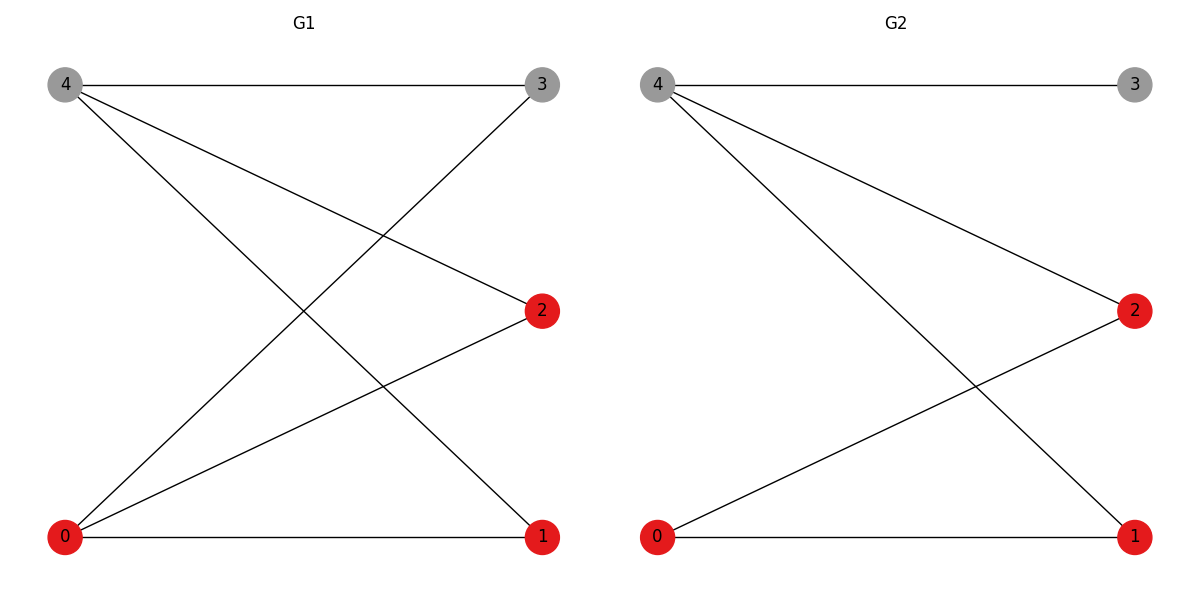
\includegraphics[width=0.6\textwidth]{../graphs/th1_3a.png}
        \label{fig:th1_3a}
      \end{figure}
      \(mod_{\mathcal{A}}(G1) = -0.0138888889\), \(mod(G2) = 0.08\)

      \item Jeśli \(s = 1\) i \(t \geq 4\) oraz \(s \geq 2\) i \(t \geq 3\) to \(\delta^{+}(G) = 1\). W pozostałych przypadkach \(\delta^{+}(G) = \infty\).
      \begin{figure}[H]
        \centering
        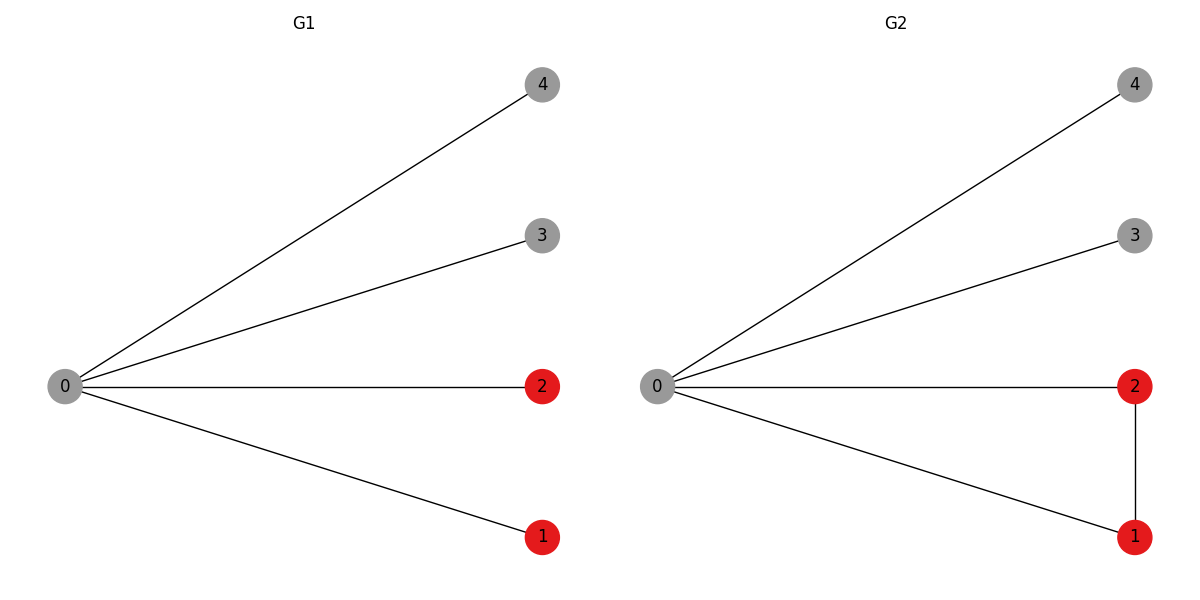
\includegraphics[width=0.6\textwidth]{../graphs/th1_3b.png}
        \label{fig:th1_3b}
      \end{figure}
      \(mod_{\mathcal{A}}(G1) = -0.125\), \(mod(G2) = 0.08\)
      \begin{figure}[H]
        \centering
        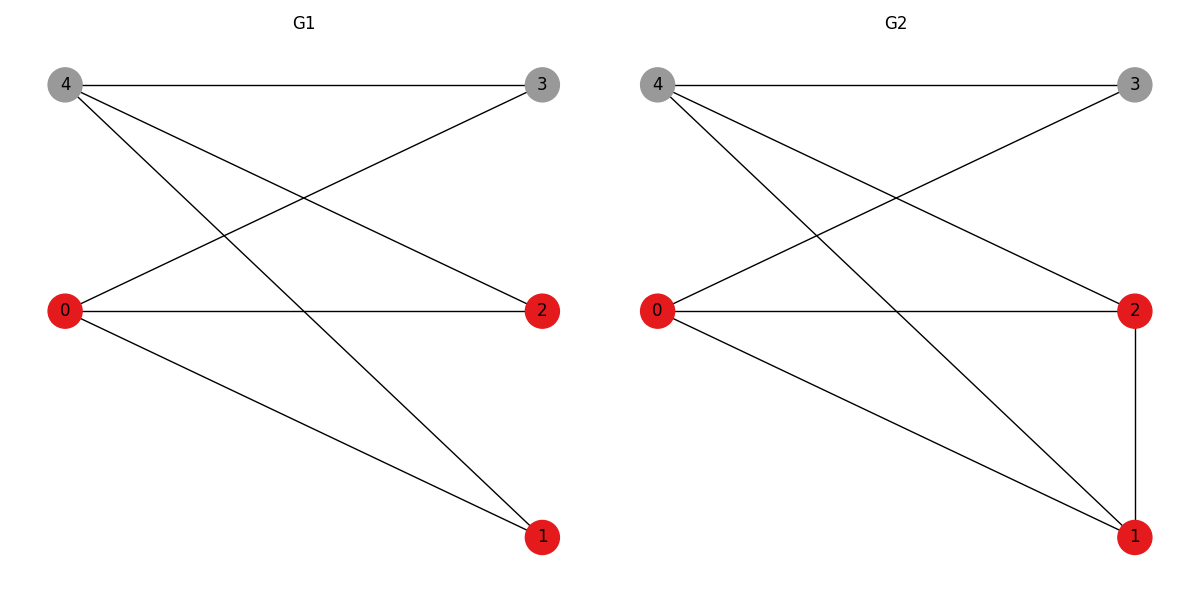
\includegraphics[width=0.6\textwidth]{../graphs/th1_3bb.png}
        \label{fig:th1_3bb}
      \end{figure}
      \(mod_{\mathcal{A}}(G1) = -0.0138888889\), \(mod(G2) = 0.0306122449\)
      \item Jeśli \(s = 1\) i \(t \geq 4\) albo \(s \geq 2\), to \(\delta(G) = 1\). Jeśli (s,t) = (1,2), to \(\delta(G) = \infty\). A gdy (s,t) = (1,3), to \(\delta(G) = 2\).
    \end{enumerate}

\end{document}